% !TEX TS-program = xelatex
\documentclass[9.0pt,a4paper]{article}
\usepackage[a4paper,top=0.82cm,bottom=0.82cm,left=1.05cm,right=1.05cm]{geometry}
\usepackage{fontspec}
\usepackage[english]{babel}
\usepackage{graphicx}
\usepackage[table]{xcolor}
\usepackage{tabularx}
\usepackage{array}
\usepackage{enumitem}
\usepackage{hyperref}
\usepackage{ragged2e}
\usepackage{microtype}
\pagestyle{empty}
\raggedbottom

% XeLaTeX typography. Font Awesome icons are vendored as vector assets in
% assets/cv/icons so the document does not depend on a system TeX icon package.
\setmainfont{Nimbus Sans}
\setsansfont{Nimbus Sans}

% Modern warm palette: brighter, happier header with high-contrast links.
\definecolor{Ink}{HTML}{1F2E33}
\definecolor{DeepLink}{HTML}{00677A}
\definecolor{Forest}{HTML}{2F8F70}
\definecolor{HeaderBg}{HTML}{FFF3E6}
\definecolor{Sage}{HTML}{EAF6F1}
\definecolor{Ivory}{HTML}{FFFEFB}
\definecolor{Copper}{HTML}{F28C28}
\definecolor{Muted}{HTML}{5B6267}
\definecolor{Rule}{HTML}{F6CBA7}
\definecolor{RoleBlue}{HTML}{005F73}
\definecolor{RoleTeal}{HTML}{287A67}
\definecolor{RoleOchre}{HTML}{985000}
\definecolor{RoleViolet}{HTML}{6750A4}

\hypersetup{colorlinks=true,urlcolor=DeepLink,linkcolor=DeepLink,citecolor=DeepLink}
\setlength{\parindent}{0pt}
\setlength{\parskip}{0pt}
\setlength{\emergencystretch}{1em}
\setlength{\tabcolsep}{0pt}
\renewcommand{\arraystretch}{1.04}
\setlist[itemize]{leftmargin=1.10em,itemsep=0.50pt,topsep=0.8pt,parsep=0pt,partopsep=0pt}
\renewcommand\labelitemi{\textcolor{Copper}{\small\raisebox{0.15ex}{\textbullet}}}
\newcolumntype{Y}{>{\RaggedRight\arraybackslash}X}

\newcommand{\cvsection}[2]{%
  \vspace{4.0pt}{\large\bfseries\color{Ink}{\textcolor{Copper}{#1}}\hspace{5pt}#2}\par
  \vspace{1pt}\textcolor{DeepLink}{\rule{0.24\linewidth}{0.78pt}}\textcolor{Copper}{\rule{0.07\linewidth}{0.78pt}}\par\vspace{2.2pt}}
\newcommand{\role}[4]{%
  \vspace{2.8pt}%
  \begin{tabularx}{\linewidth}{@{}Y r@{}}{\bfseries\color{Ink}#1} & {\bfseries\color{DeepLink}#2}\\[-0.2pt]{\itshape\color{DeepLink}#3} & {\color{Muted}#4}\\\end{tabularx}\vspace{2.2pt}}
\newcommand{\skillrow}[2]{\textbf{\color{Ink}#1} & #2\\[1.8pt]}
\newcommand{\contact}[2]{\textcolor{Copper}{#1}\hspace{3pt}#2}
\newcommand{\paper}[1]{{\small\sloppy #1\par}\vspace{1.1pt}}
\newcommand{\faicon}[1]{\raisebox{-0.12ex}{\includegraphics[height=1.05em]{icons/#1.pdf}}}
\newcommand{\githublink}[2]{\href{#2}{\textcolor{DeepLink}{\small\faicon{github}\,#1}}}
\newcommand{\weblink}[2]{\href{#2}{\textcolor{DeepLink}{\small\faicon{external-link}\,#1}}}
\newcommand{\projectline}[3]{\textbf{\color{Ink}#1}\hspace{3pt}#3 --- #2\par}

\begin{document}
\color{Ink}\fontsize{8.74}{9.94}\selectfont

% Header: light, high contrast, link labels visible.
\noindent\colorbox{HeaderBg}{%
\parbox{\dimexpr\linewidth-2\fboxsep}{%
\begin{minipage}[c]{0.785\linewidth}
\vspace{4pt}
{\fontsize{20.8}{22.4}\selectfont\bfseries\color{Ink} Dr. Chilperic Armel Foko Kuate}\par
\vspace{1.6pt}{\fontsize{9.2}{10.3}\selectfont\bfseries
\textcolor{RoleBlue}{Computational Scientist}\;|\;\textcolor{RoleTeal}{Multiscale Modeller}\par
\textcolor{RoleOchre}{Scientific Software Developer}\;|\;\textcolor{RoleViolet}{Applied Mathematics}}\par
\vspace{2.2pt}{\fontsize{8.35}{9.2}\selectfont\color{Muted} Mechanistic models \textbullet\ numerical simulation \textbullet\ inference and optimisation \textbullet\ scientific software \textbullet\ reproducible evidence}\par
\vspace{2.8pt}{\fontsize{8.45}{9.35}\selectfont
\contact{\faicon{location-dot}}{Düsseldorf, Germany}\hspace{7pt}
\contact{\faicon{phone}}{+49 176 55 20 83 05}\hspace{7pt}
\contact{\faicon{envelope}}{\href{mailto:chilpericarmel@gmail.com}{chilpericarmel@gmail.com}}}\par
\vspace{2.1pt}{\fontsize{8.45}{9.35}\selectfont
\contact{\faicon{github}}{\href{https://github.com/chilperic}{github.com/chilperic}}\hspace{6pt}
\contact{\faicon{globe}}{\href{https://chilperic.github.io}{chilperic.github.io}}}\par
\vspace{2.1pt}{\fontsize{8.45}{9.35}\selectfont
\href{https://orcid.org/0000-0002-0140-7588}{\textcolor{DeepLink}{\textbf{ORCID} 0000-0002-0140-7588}}\hspace{6pt}
\href{https://scholar.google.com/citations?user=tOGuNMkAAAAJ}{\textcolor{DeepLink}{\textbf{Scholar} profile}}}\par
\vspace{4pt}
\end{minipage}\hfill
\begin{minipage}[c]{0.16\linewidth}
\centering
\fcolorbox{Copper}{white}{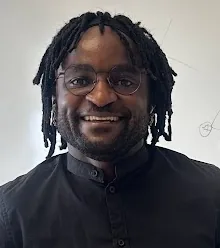
\includegraphics[width=2.35cm,height=2.66cm,keepaspectratio]{profile_picture.png}}
\end{minipage}
}}

\vspace{5pt}
\cvsection{\faicon{user}}{Profile}
\begin{itemize}
  \item Computational scientist and multiscale modeller with a PhD in Quantitative and Theoretical Biology and formal training in applied mathematics; research spans cell populations, metabolic networks, and coupled plant--environment physiology.
  \item Build interpretable mechanistic models and numerical workflows using ODE/DAE and stochastic systems, nonlinear dynamics, parameter estimation, optimisation, sensitivity, uncertainty, and identifiability analysis.
  \item Develop reproducible scientific software, including FokoLab, a browser-native modelling platform designed around user-defined models, simulation, analysis, diagnostics, visualisation, and exportable evidence.
\end{itemize}

\cvsection{\faicon{cubes}}{Multiscale modelling and computational science}
\begin{tabularx}{\linewidth}{@{}p{0.25\linewidth}Y@{}}
\textbf{Across biological scales} & Enzyme kinetics and metabolic networks; cellular population dynamics; organ/leaf biochemistry, heat balance and hydraulics; environmental forcing and adaptive phenotypes.\\[2pt]
\textbf{Applied mathematics} & Nonlinear dynamical systems, stability and bifurcation reasoning, stochastic processes, branching processes, inverse problems, constrained optimisation, and numerical analysis.\\[2pt]
\textbf{Inference \& validation} & Parameter fitting, identifiability, Sobol/Morris sensitivity, uncertainty analysis, simulation ensembles, numerical reference checks, and explicit limits of interpretation.\\[2pt]
\textbf{Scientific software} & Reproducible Python and browser-native modelling tools with editable inputs, diagnostics, visualisation, testing, documentation, and data/report export.\\
\end{tabularx}

\cvsection{\faicon{wrench}}{Core methods and tools}
\begin{tabularx}{\linewidth}{@{}p{0.22\linewidth}Y@{}}
\skillrow{Modelling}{ODE/DAE systems, kinetic rate laws, energy and hydraulic balances, nonlinear dynamics, stochastic processes, branching processes, master equations.}
\skillrow{Numerics}{NumPy/SciPy, CVODE/SUNDIALS, CasADi/IPOPT, Pyomo, lmfit, CMA-ES, parameter fitting, constrained optimisation.}
\skillrow{Analysis}{Sobol/Morris sensitivity, identifiability, uncertainty analysis, simulation ensembles, stability analysis, PCA/statistical diagnostics.}
\skillrow{Programming}{Python, Julia, R, MATLAB; JavaScript/HTML/CSS for browser-native scientific software.}
\skillrow{Workflow}{Git/GitHub, Jupyter, Linux, HPC exposure, testing, LaTeX, reproducible pipelines, technical documentation.}
\end{tabularx}

\cvsection{\faicon{briefcase}}{Research and modelling experience}
\role{Independent Computational Scientist \& Scientific Software Developer}{Nov 2025--Present}{Düsseldorf, Germany}{}
\begin{itemize}
  \item Architect and develop FokoLab, a browser-native scientific modelling platform spanning deterministic and stochastic dynamics, optimisation, sensitivity, population/evolution, statistics/ML, symbolic analysis, reproducibility and validation diagnostics.
  \item Refactor research code into documented, testable repositories with explicit model assumptions, numerical checks, reusable examples, and reproducible computational workflows.
  \item Advance two first-author manuscripts on multiscale modelling of plant adaptation across the C3--C4 continuum while completing a professional German B2 programme.
\end{itemize}

\role{Postdoctoral Researcher}{Nov 2022--Oct 2025}{CEPLAS / Institute of Computational Cell Biology, HHU Düsseldorf}{Germany}
\begin{itemize}
  \item Developed a multiscale thermo-hydraulic-biochemical framework coupling C3/C4 carbon assimilation, mesophyll/bundle-sheath heat balance, stomatal conductance, water transport, soil state, irradiance, humidity, and temperature-dependent enzyme kinetics.
  \item Combined Sobol sensitivity, simulation ensembles, and CMA-ES optimisation across contrasting climates to identify influential traits, physiological trade-offs, and environment-specific adaptive strategies.
  \item Worked with experimental collaborators and supervised 2 MSc and 2 BSc projects, translating biological questions into quantitative models and interpretable computational analyses.
\end{itemize}

\newpage
\cvsection{\faicon{briefcase}}{Research and modelling experience --- continued}
\role{Marie Sk{\l}odowska-Curie PhD Researcher}{Aug 2019--Aug 2022}{Institute of Quantitative and Theoretical Biology, HHU Düsseldorf}{Germany}
\begin{itemize}
  \item Developed two ODE-based models of hepatic fatty-acid metabolism and de novo synthesis, connecting qualitative dynamical-systems analysis with quantitative simulation of experimental time courses.
  \item Derived conditions for metabolic bistability using polynomial/root analysis and stability theory; fitted semi-mechanistic enzyme-kinetic models and assessed robustness with sensitivity analysis.
  \item Contributed enzyme-kinetic formalism to a cross-institutional differentiable constraint-based modelling framework; work published in \textit{Bioscience Reports} and \textit{Metabolic Engineering}.
\end{itemize}

\role{Research Fellow}{Nov 2017--Mar 2019}{AIMS Cameroon and AIMS Rwanda}{Cameroon / Rwanda}
\begin{itemize}
  \item Developed stochastic and deterministic models of T-cell proliferation using branching-process, master-equation, delay and compartmental formulations.
  \item Built likelihood-based fitting workflows for CFSE-type data and extracted interpretable cell-population parameters from experimental distributions.
  \item Delivered 200+ teaching hours in mathematical modelling, ODEs, stochastic processes, algebra, and Python.
\end{itemize}

\cvsection{\faicon{puzzle-piece}}{Selected projects}
\projectline{FokoLab}{Browser-native scientific modelling platform for user-defined models, simulation, fitting, sensitivity, optimisation, population/evolution, diagnostics, visualisation and reproducible export.}{\weblink{Open platform}{https://chilperic.github.io/chilperic_ode_solver/index.html}}
\projectline{Photosynthesis climate-adaptation model}{Python/CasADi mechanistic model coupling C3/C4 biochemistry, heat balance, hydraulics, soil state, climate forcing, optimisation, and sensitivity workflows.}{\githublink{GitHub}{https://github.com/chilperic/photosynthesis-climate-adaptation-model}}
\projectline{Fatty-acid de novo synthesis model}{Kinetic ODE model with enzyme-rate laws, parameter estimation, validation, and sensitivity analysis.}{\githublink{GitHub}{https://github.com/chilperic/fatty-acid-denovo-synthesis-model}}
\projectline{Fatty-acid metabolism bistability}{Nonlinear metabolic model exploring switching behaviour, steady states, and robustness in lipid metabolism.}{\githublink{GitHub}{https://github.com/chilperic/fatty-acid-metabolism-bistability}}
\projectline{Master work: T-cell proliferation models}{AIMS Ghana MSc thesis, \textit{Reverse-engineering of T-cell proliferation dynamics}: Smith--Martin DDE, Cyton model, branching-process thinking, CFSE-type fitting, and population-response inference.}{\githublink{GitHub}{https://github.com/chilperic/tcell-proliferation-models}}

\cvsection{\faicon{graduation-cap}}{Education}
\begin{tabularx}{\linewidth}{@{}p{0.17\linewidth}Y@{}}
\textbf{2019--2023} & \textbf{PhD, Quantitative and Theoretical Biology}, Heinrich Heine University Düsseldorf. Dissertation: dynamic computational modelling of fatty-acid synthesis and metabolism; defended March 2023. Supervisor: Prof. Dr. Oliver Ebenhöh.\\[2pt]
\textbf{2017--2019} & \textbf{Master 2, Mathematics and Applications}, University of Yaoundé I. Advanced numerical analysis, dynamical systems, inverse problems.\\[2pt]
\textbf{2015--2016} & \textbf{MSc, Mathematical Sciences}, AIMS Ghana. Thesis: \textit{Reverse-engineering of T-cell proliferation dynamics}; Smith--Martin DDE, Cyton model, CFSE-type data, and population-dynamics inference.\\[2pt]
\textbf{2009--2012} & \textbf{BSc, Mathematics}, University of Douala. Algebra, analysis, geometry.\\
\end{tabularx}

\cvsection{\faicon{book}}{Selected publications}
\paper{Dourado, V.H., \textbf{Foko Kuate, C.A.}, Liebermeister, W., Lercher, M.J. Growth mechanics and the emergence of metabolic oscillations in growing cells. \textit{bioRxiv} preprint, 2025. DOI: 10.1101/2025.06.24.661369. Second author; contributed mathematical framework for metabolic-oscillation modelling.}
\paper{\textbf{Foko Kuate, C.A.}, Ebenhöh, O., Bakker, B.M., Raguin, A. Kinetic data for modeling the dynamics of the enzymes involved in animal fatty-acid synthesis. \textit{Bioscience Reports}, 43(7), BSR20222496, 2023. DOI: 10.1042/BSR20222496.}
\paper{Wilken, S.E., Besançon, M., Kratochvíl, M., \textbf{Foko Kuate, C.A.}, Trefois, C., Gu, W., Ebenhöh, O. Interrogating the effect of enzyme kinetics on metabolism using differentiable constraint-based models. \textit{Metabolic Engineering}, 74, 72--82, 2022. DOI: 10.1016/j.ymben.2022.09.002.}
\paper{Two first-author manuscripts in preparation on mechanistic modelling of plant adaptation across the C3--C4 continuum.}

\cvsection{\faicon{certificate}}{Training, leadership, languages, awards}
\begin{tabularx}{\linewidth}{@{}p{0.19\linewidth}Y@{}}
\textbf{Training} & Bayer B4U University Mentoring Programme, completed 2025 (mentor: Benjamin Buer); PoLiMeR Marie Curie ITN doctoral training; Advanced AI and Data Science Workshop, HeiCAD; Hands-on Course on Optimal Control with CasADi.\\[2pt]
\textbf{Leadership} & C4 Plant Project Group Leader; Early Career Researchers' Representative, Marie Curie ITN; supervised 2 MSc and 2 BSc projects.\\[2pt]
\textbf{Languages} & French: native; English: fluent; German: B1+ (currently completing B2 Berufssprachkurs; exam expected Nov 2026).\\[2pt]
\textbf{Awards} & Marie Sk{\l}odowska-Curie ITN Fellowship (PoLiMeR); Post-AIMS Research Bursary; F.K.A. Allotey Meritorious Award, AIMS Ghana.\\
\end{tabularx}

\end{document}
